\begin{frame}{Signal VS WhatsApp VS Telegram}
    \framesubtitle{Telegram}
    
    \textbf{Pro}
    \begin{itemize}
        \item Sicurezza: autenticazione a due fattori
        \item Supporta file di qualsiasi dimensione
        \item Eliminazione automatica dell'account se inutilizzato per troppo tempo
        \item Interfaccia personalizzabile
    \end{itemize}\pause

    \textbf{Contro}
    \begin{itemize}
        \item Crittografia end-to-end solo per chat segrete, non per chat individuali e di gruppo
        \item Chat cloud che utilizzano la crittografia client-server: l’azienda ha accesso ai messaggi
        \item Usa GPS per trovare utenti nelle vicinanze 
    \end{itemize}

    \note{
        Informazioni raccolte: indirizzo IP, dispositivi, cronologia dei nomi utente e contatti.\newline
        Messaggi crittografati sul dispositivo utente ma decrittati sui server, ri-crittografati e poi inviati al destinatario per essere decrittati in modo definitivo. Telegram possiede le chiavi lato server e può teoricamente accedere al contenuto dei messaggi.\newline
        Telegram garantisce di non aver condiviso ad oggi alcun dato con terze parti e/o enti governativi.
    }
\end{frame}

\begin{frame}{Signal VS WhatsApp VS Telegram}
    \framesubtitle{Telegram}

    Mentre Signal e WhatsApp utilizzano implementazioni del protocollo Signal, Telegram utilizza il protocollo proprietario \textbf{MTProto} per la crittografia dei messaggi.\newline\pause
    Essendo a implementazione closed-source non permette l'analisi completa da parte dei ricercatori.\newline

    \note{
        In ambito crittografico è considerata buona norma utilizzare protocolli e algoritmi verificati da un numero di ricercatori o esperti maggiore possibile.\\
        Ciò si contrappone alla logica di \textit{security through obscurity} che invece vorrebbe che i protocolli siano tanto più sicuri quanto meno sono stati analizzati.\\
        Per questo motivo protocolli open-source sono in genere preferibili, in quanto è più probabile che vengano rilevati eventuali bug in protocolli analizzati da team più ampi e numerosi.
    }
\end{frame}

\begin{frame}{Signal VS WhatsApp VS Telegram}
    \framesubtitle{Telegram}

    \begin{figure}
        \centering
        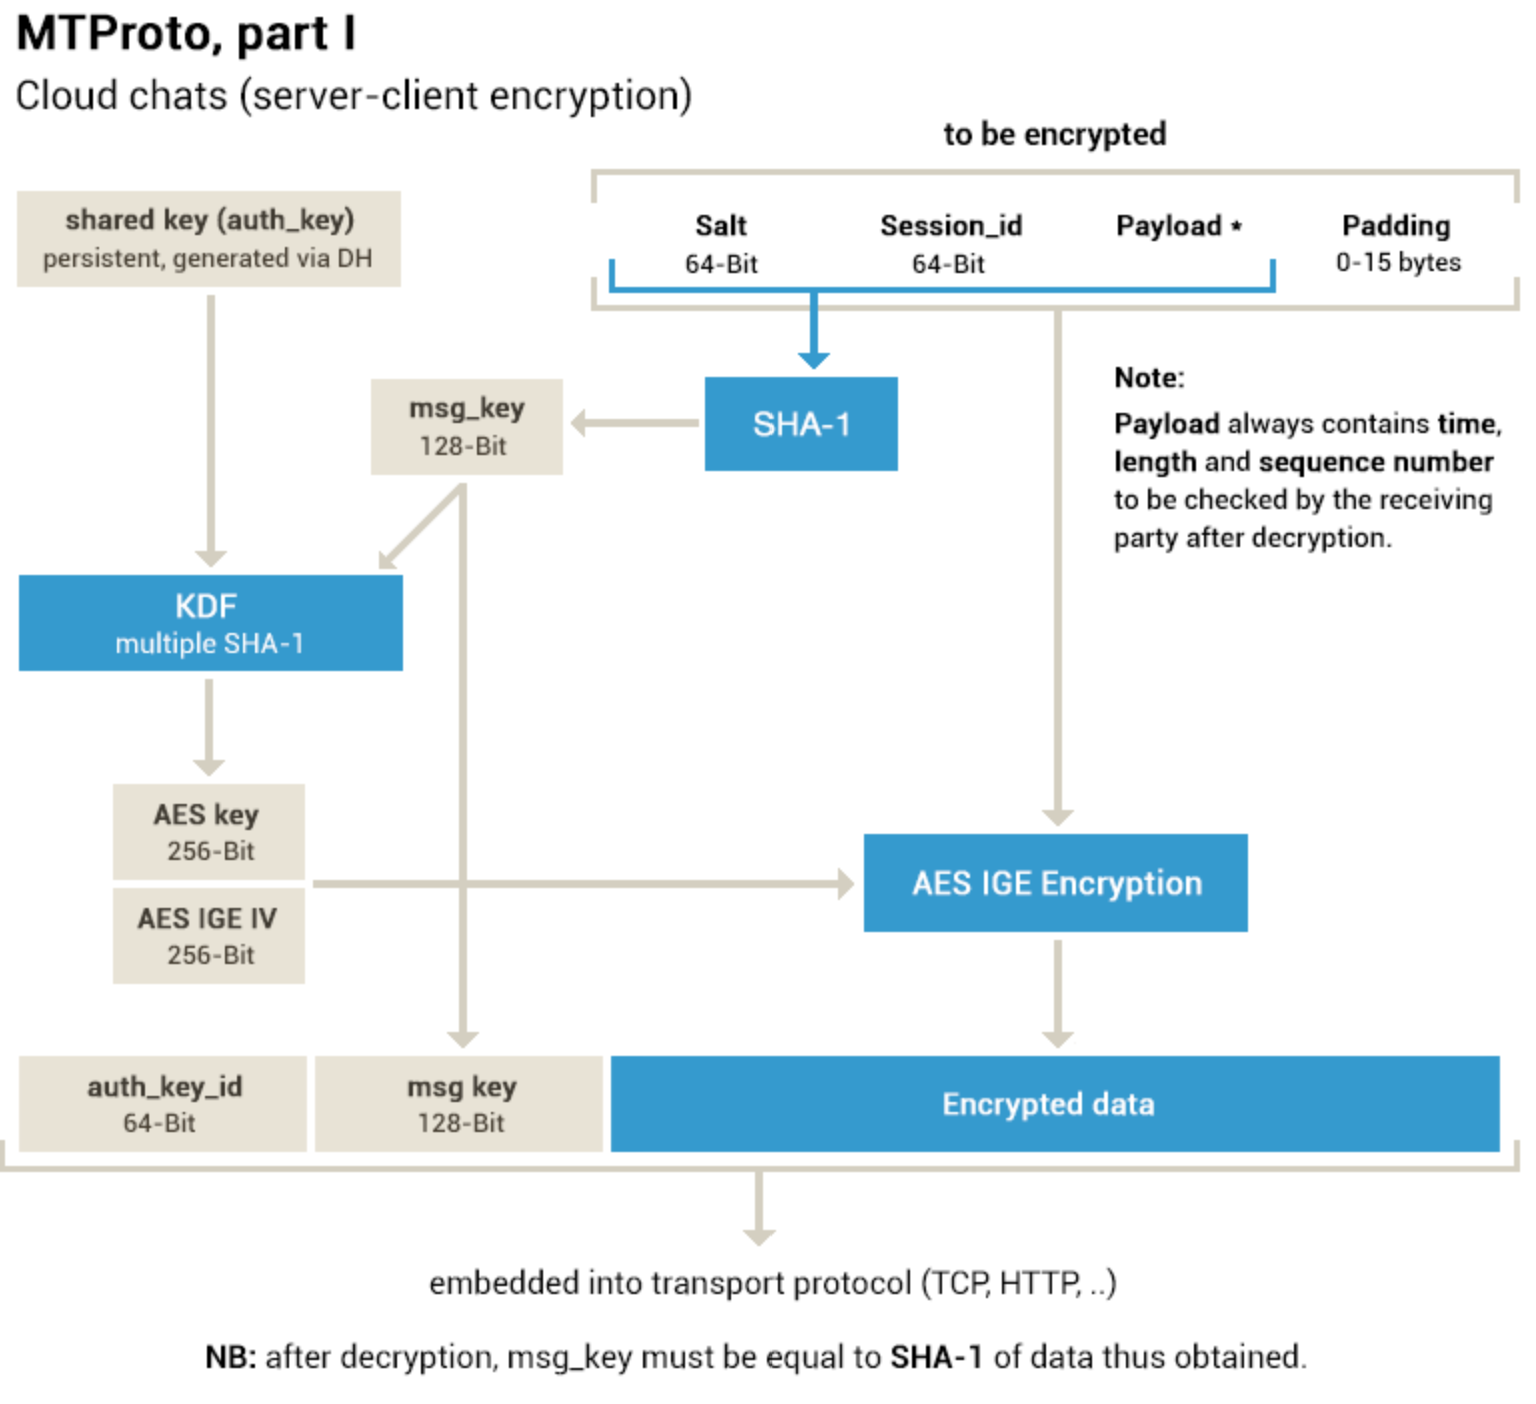
\includegraphics[width=0.5\textwidth]{mtproto.png}
        \caption{MTProto}
        \label{tag: mtproto}
    \end{figure}    

    \note{
        Il salt, $session\_id$ e $payload$ del messaggio vengono crittografati con $SHA-1$ a creare una $msg\_key$.

        La $msg\_key$ viene usata insieme alla $auth\_key$ come input di una $KDF$ che restituisce una chiave $AES$ e un vettore di inizializzazione da utilizzare a loro volta come input di una funzione $AES$ $IGE$ $Encryption$.

        Da quest'ultima funzione si ottengono i dati crittografati, ai quali vengono aggiunti $auth\_key\_id$ al fine di identificare l'utente e $msg\_key$. 

        Al fine di autenticare il messaggio, una volta decodificato viene comparata la $msg\_key$ ricevuta con quella computata localmente.\cite{telegramdoc}
    }
\end{frame}
